\documentclass[12pt]{article}

\usepackage{graphicx}
\usepackage{epstopdf}


\usepackage[spanish]{babel} % silabea palabras castellanas <- Puedo poner comentarios para explicar de que va este comando en la misma línea
\selectlanguage{spanish} 

%Encoding
\usepackage[utf8]{inputenc} % Acepta caracteres en castellano
\usepackage[T1]{fontenc} % Encoding de salida al pdf

%Triunfó el mal
\usepackage[normalem]{ulem}
\useunder{\uline}{\ul}{}
\providecommand{\e}[1]{\ensuremath{\times 10^{#1}}}
\usepackage{quotmark} %Uso consistente con la RAE de comillas
\usepackage{listings} % Comandos de la terminal

\usepackage{textcomp}
\usepackage{gensymb}


%Hipertexto
\usepackage[colorlinks=true,urlcolor=blue,linkcolor=blue]{hyperref} % navega por el doc: hipertexto y links

%Aquello de las urls
\usepackage{url} 

%simbolos matemáticos
\usepackage{amsmath}
\usepackage{amsfonts}
\usepackage{amssymb}
\usepackage{physics} %Best pack

% permite insertar gráficos, imágenes y figuras, en pdf o en eps
\usepackage{graphicx}
\usepackage{epstopdf}
\usepackage{multirow}
\usepackage{float}
\usepackage[export]{adjustbox}
% geometría del documento, encabezados y pies de páginas, márgenes
\usepackage{geometry}
\usepackage{comment}

%\usepackage[english]{babel}
%\usepackage[latin5]{inputenc}
% \usepackage{hyperref}
%\newdate{date}{10}{05}{2013}
%\date{\displaydate{date}}
\begin{document}
\title{Cúmulos Abiertos \\ Taller 5 Diagrama HR de Cúmulos Estelares (CLEA)}

\author{
\textbf{Javier Alejandro Acevedo Barroso\thanks{e-mail: \texttt{ja.acevedo12@uniandes.edu.co}}}\\
\textit{Universidad de los Andes, Bogotá, Colombia}\\
 }% Hasta aquí llega el bloque "author" (son dos autores por informe, orden alfabético)

\date{\today}
%\date{Versión $\alpha \beta$ fecha del documento}
\maketitle %Genera el título del documento


\normalsize
\newpage


\section{Diagrama de Hertzsprung–Russell (HR)}
Son gráficas de magnitud contra color (B- V) para una población estelar dada.
La idea detrás de estos diagramas es que permiten una rápida clasificación de las estrellas por color, pues el color se relaciona con la temperatura superficial; y permite saber la edad de una población estelar, pues de acuerdo a los modelos de formación estelar, podemos obtener diagramas HR teóricos para cúmulos de diferentes edades.
En un diagrama HR se pueden identificar diferentes líneas de acuerdo al tipo de reacción nuclear que ocurre en la estrella.
A las estrellas que fusionan hidrógeno se les denomina estrellas en la secuencia principal, y representan tanto la mayoría de estrellas como la línea más larga. En la figura \ref{diag} se puede observar las diferentes líneas de un diagrama HR.



\begin{figure}[H]
  \centering
   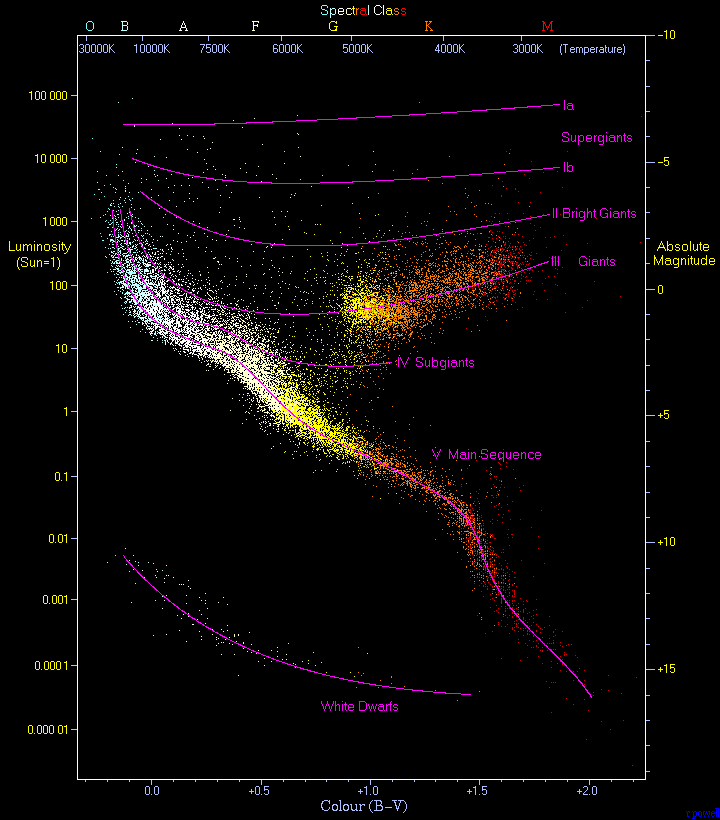
\includegraphics[width= 4.20in]{HRdiag.png}
  \caption{Diagrama HR de 22000 estrellas del catálogo HIPPARCOS.\cite{hrdiag}  }
  \label{diag}
\end{figure}


\section{Ejercicio de CLEA: diagrama HR de cúmulos estelares}
El objetivo del ejercicio es aprender a utilizar el software \tqt{Virtual Educational Observatory} (VIREO), que es un observatorio virtual que permite generar imágenes astronómicas simuladas.
El observatorio se vale de catálogos astronómicos y bases de datos para producir imágenes simuladas de instrumentos CCD o espectrógrafos a través de telescópios.
Las imágenes generadas son en formato FITS.
Los objetivos específicos del ejercicio son generar diagramas HR para diferentes cúmulos estelares, determinar la edad del cúmulo y la distancia al mismo usando los diagramas HR.

El primer paso del ejercicio es instalar y ejecutar el software de VIREO\footnote{Se encuentra disponible en \url{http://www3.gettysburg.edu/~marschal/clea/Vireo.html} Note que el software ya no recibe actualizaciones.}.
Una vez instalado VIREO, se procede a iniciar el ejercicio \tqt{HR Diagrams of Stars Clusters}. Después, se puede seleccionar datos de diferentes cúmulos y obtener su diagrama HR, ver figura \ref{vireaohr}

\begin{figure}[H]
  \centering
   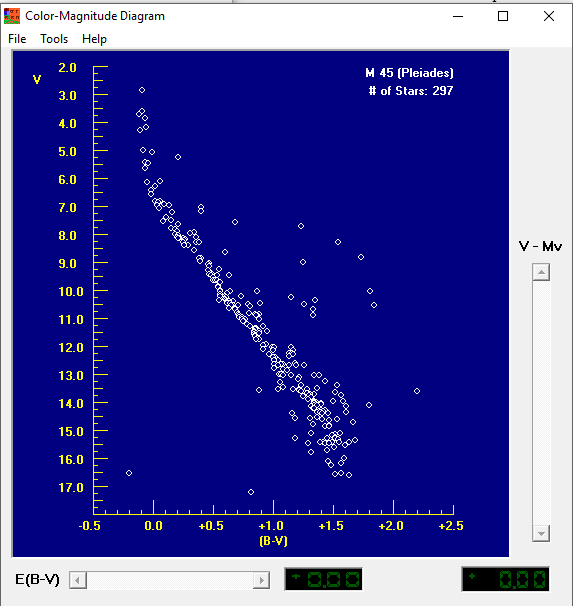
\includegraphics[width= 3.40in]{hrvireo.png}
  \caption{Diagrama HR del cúmulo M45 Las Pleiades. Note que la mayoría de estrellas se encuentran en la secuencia principal.}
  \label{vireaohr}
\end{figure}

Ahora, el color y la magnitud absoluta de una población estelar en la secuencia principal han sido bien caracterizados por astrónomos a través de observación y modelamiento. VIREO permite acceder la curva de la secuencia principal con color y magnitud absoluta, a esta curva se le denomina secuencia principal de edad cero. Igualmente, VIREO permite ajustar la  curva de edad cero para obtener el módulo de la distancia y el exceso de color. Esto se puede ver en la figura \ref{edadCero}.


\begin{figure}[H]
    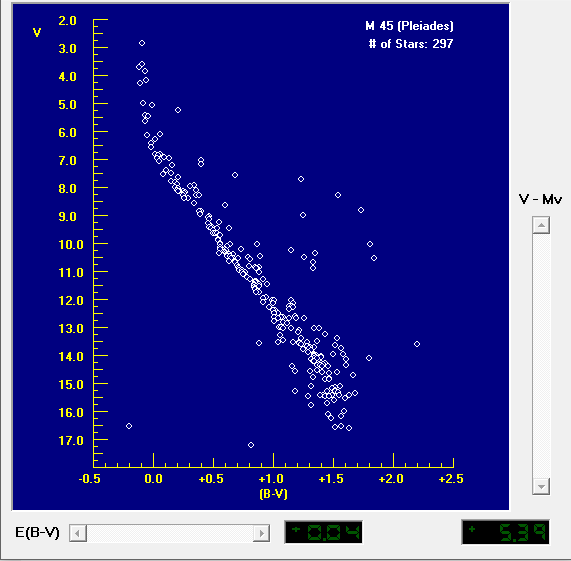
\includegraphics[width= 3.40in]{plea0.png}
    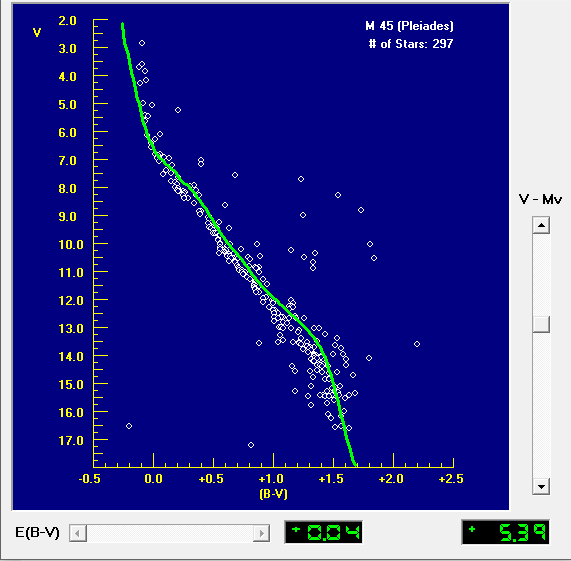
\includegraphics[width= 3.40in]{plea1.png}
  \caption{Izquierda: diagrama HR del cúmulo M45 Las Pleiades. Derecha: diagrama HR junto a la curva de edad cero ajustada para el cúmulo M45, implicando un modulo de distancia $m - M = 5.39$ y un exceso de color $E(B-V) = 0.04$}
  \label{vireaohr}
\end{figure}


Para determinar la edad de un cúmulo nos valemos de que los diferentes tipos de estrella evolucionan a diferentes velocidades. En particular, a medida que pasa el tiempo, las estrellas más calientes y masivas (la parte superior de la secuencia principal) queman su combustible y se mueven a la derecha del diagrama, a la sección de supergigantes rojas.
A medida que avanza el tiempo, estrellas cada vez menos masivas queman su combustible y se mueven a la sección de gigantes rojas, de modo que la secuencia principal se convierte en una \tqt{mecha} que mide la edad del cúmulo.
A la curva teórica de un diagrama HR para una población estelar de una edad dada se le conoce como \emph{isocrona}. En la figura \ref{hrmetal} se puede apreciar dos curvas isocronas para el cúmulo M45 con diferentes metalicidades.

\begin{figure}[H]
    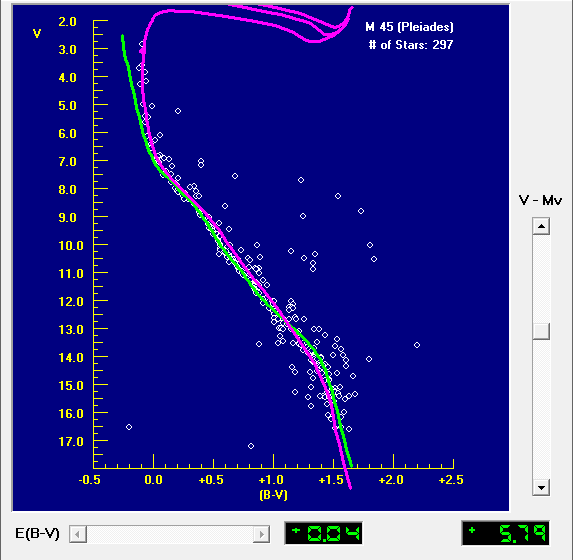
\includegraphics[width= 3.40in]{plea2.png}
    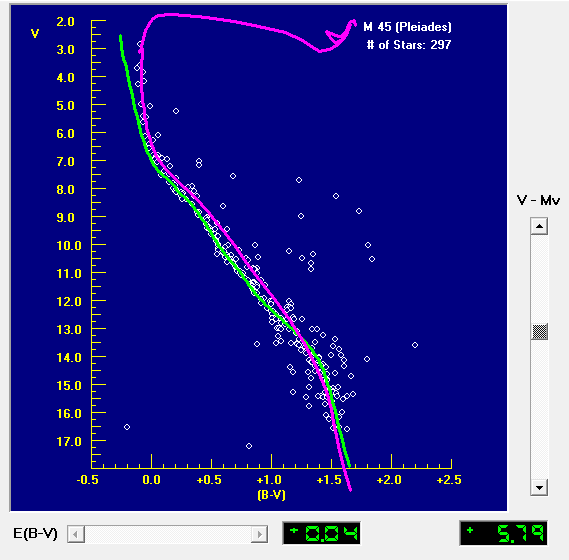
\includegraphics[width= 3.40in]{plea3.png}
  \caption{Izquierda: diagrama HR del cúmulo M45 Las Pleiades con isocrona (purpura) de metallicidad similar a la metalicidad en el vecindario solar. Derecha: diagrama HR del cúmulo M45 ahora con $40\%$ más metallicidad.}
  \label{hrmetal}
\end{figure}

Ahora, se generará diagramas HR para los cúmulos: \tqt{NCG 752}, \tqt{Mel 20}, \tqt{M45}, \tqt{Hyades}, \tqt{M44},\tqt{M67},  \tqt{IC 4665}, se ajustará la curva de edad cero para determinar su exceso de color $E(B-V)$ y su módulo de distancia. Y por último, se ajustará una isocrona para determinar la edad del cúmulo. 

Recuerde que para obtener la distancia a un objeto a partir de su módulo de distancia de puede usar:
\begin{equation}
m- M = 5\log{d} - 5    
\end{equation}
Donde $d$ es la distancia al objeto en Parsecs.
En las siguientes figuras se presentan las gráficas HR de los cúmulos con sus respectiva curvas ajustadas:
\newpage

\begin{figure}[H]
    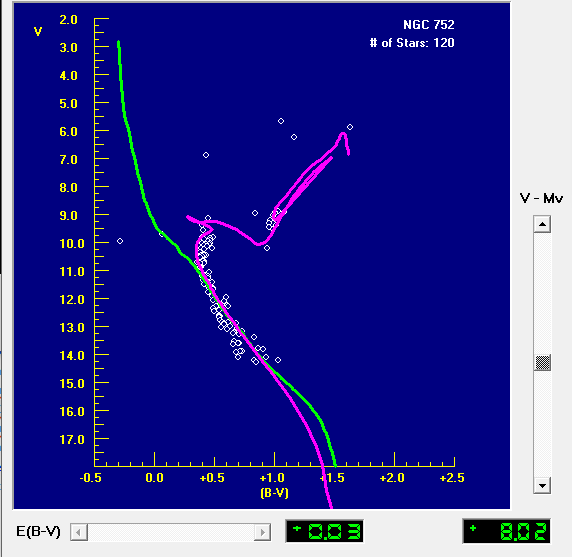
\includegraphics[width= 3.40in]{ngc752.png}
    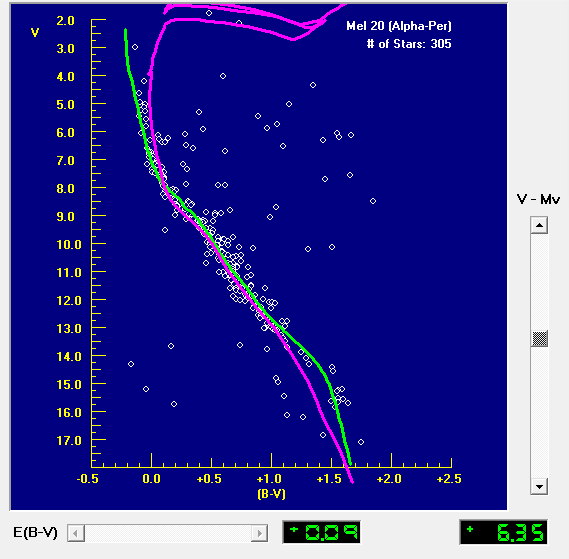
\includegraphics[width= 3.40in]{mel20.png}
  \label{hrmetal}
\end{figure}
\begin{figure}[H]
    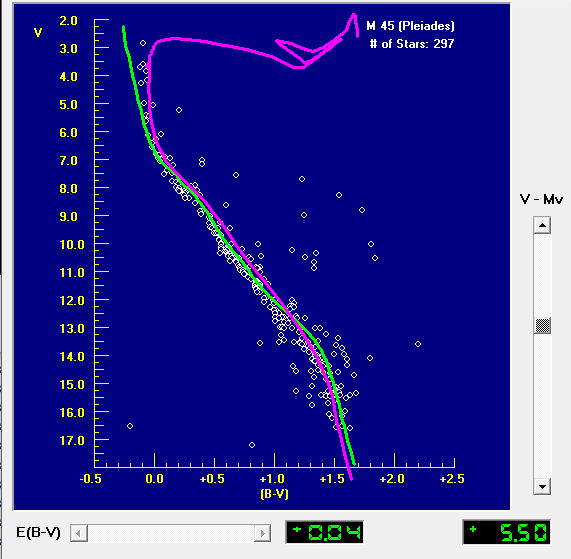
\includegraphics[width= 3.40in]{M45.png}
    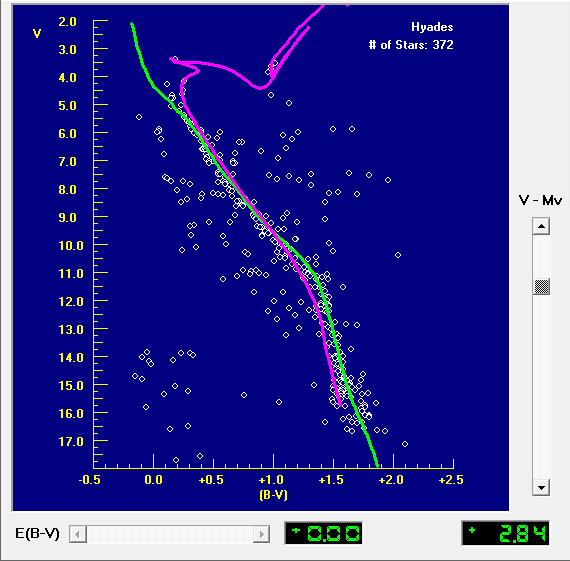
\includegraphics[width= 3.40in]{hyades.png}
  \label{hrmetal}
\end{figure}

\begin{figure}[H]
    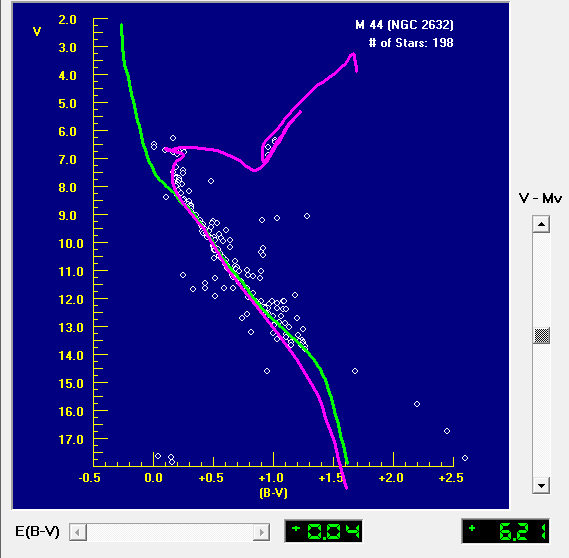
\includegraphics[width= 3.40in]{M44.png}
    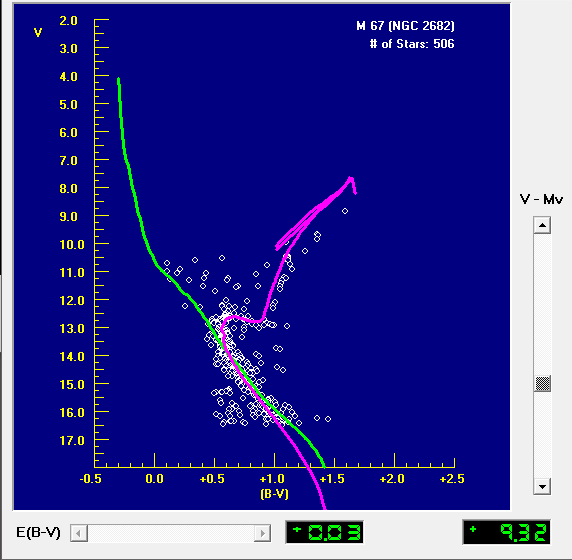
\includegraphics[width= 3.40in]{M67.png}
  \label{hrmetal}
\end{figure}
\begin{figure}[H]
    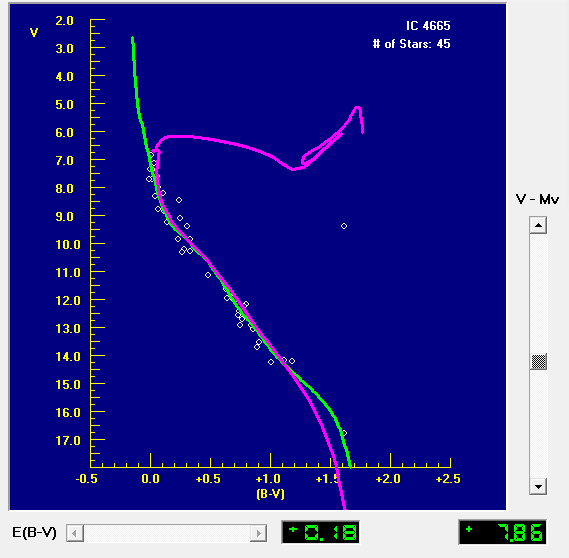
\includegraphics[width= 3.40in]{ic4665.png}
    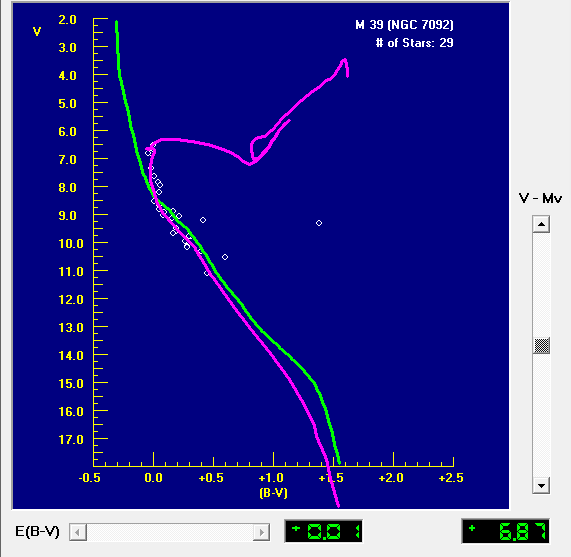
\includegraphics[width= 3.40in]{M39.png}
  \label{hrmetal}
\end{figure}


\newpage
En la tabla a continuación se encuentran los datos calculados de los cúmulos:

\begin{table}[htb]
    \centering
    \label{tabla}
	\begin{tabular}{|c|c|c|c|c| }
	\hline
	Cúmulo & $E(B-V)$ & $m-M$ & Distancia [$pcs$] & Edad del cúmulo [millones de años]  \\ \hline
	NCG 752 & -0.03 & 8.02 & 401.79 & 1259  \\ \hline
	Mel 20 & +0.09 & 6.35 & 186.2 & 63  \\ \hline
	M45 & +0.04 & 5.50 & 125.89 & 126  \\ \hline
	Hyades & 0.00 & 2.84 & 36.98 & 891  \\ \hline
	M44 & +0.04 & 6.21 & 174.58 & 794  \\ \hline
	M67 & -0.03 & 9.32 & 731.14 & 5623  \\ \hline
	IC 4665 & 0.18 & 7.86 & 373.25 & 224  \\ \hline
	M39 & +0.01 & 6.87 & 238.78 & 447  \\ \hline
	\end{tabular}
\end{table}

Se concluye que el cúmulo más próximo es el cúmulo de Hyades a tan solo 37 Parsecs de la Tierra. El cúmulo más lejano es el cúmulo M67 a 731 Parsecs de nosotros. Se observa que la mayoría de los cúmulos son mucho menores que el Sol (que tiene aproximadamente 4600 millones de años), implicando que probablemente se formaron mucho después de la formación de la galaxia. La baja edad de los cúmulos también se observa en la metalicidad de las curvas isocronas. Exceptuando el cúmulo M67, la mayoría de los cúmulos tenían metalicidad cercana a la del Sol. El cúmulo más jóven es Mel 20 con solo 63 millones de años de edad. El cúmulo más antiguo es el cúmulo M67 con 5623 millones de años.



















\bibliography{bibte}
\bibliographystyle{plain}


\end{document}




\begin{figure}[H]
  \centering
   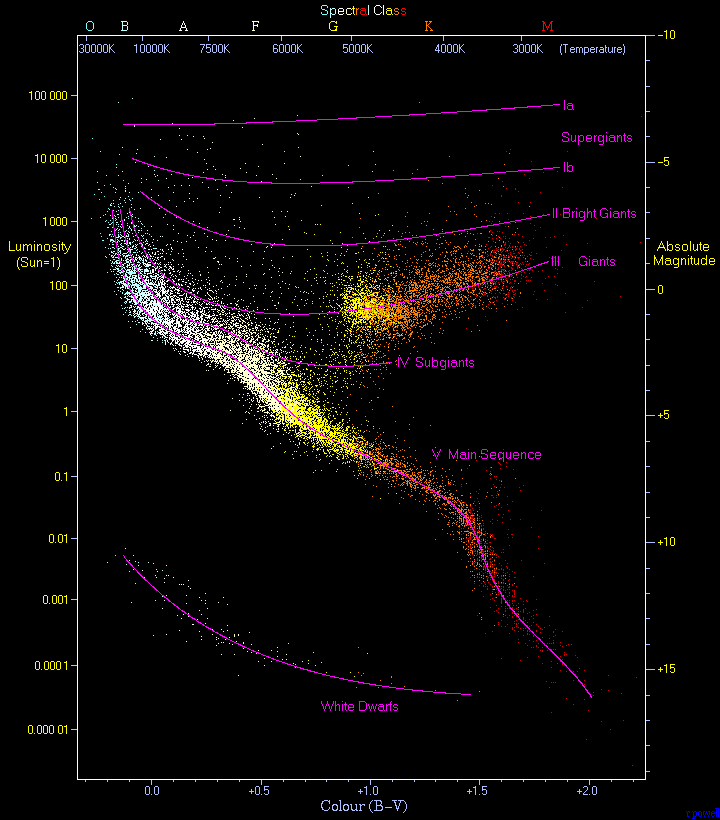
\includegraphics[width= 4.20in]{HRdiag.png}
  \caption{Diagrama HR de 22000 estrellas del catálogo HIPPARCOS.\cite{hrdiag}  }
  \label{diag}
\end{figure}






\section{Cronograma}

\begin{table}[htb]
	\begin{tabular}{|c|cccccccccccccccc| }
	\hline
	Tareas $\backslash$ Semanas & 1 & 2 & 3 & 4 & 5 & 6 & 7 & 8 & 9 & 10 & 11 & 12 & 13 & 14 & 15 & 16  \\
	\hline
	1 & X & X & X  &   &   &   &   &  &  &   &   &   &   &   &   &   \\
	2 &   &  & X & X & X &  &  &   &   &  &  &  &   &  &  &   \\
	3 &   &   &   &  & X  & X  & X  & X &   &   &   &  &   &   &  &   \\
	4 &  &  &  &  &  &  &  & X & X & X & X &   &   &   &   &   \\
    5 &  &  &  &  &  &  & X & X &  &  &  &   &   &   &   &   \\
	6 &   &   &   &   &  &   &  X & X  &  &   &  X & X &  X & X  & X &   \\
	\hline
	\end{tabular}
\end{table}
\vspace{1mm}
%CCDRED se encarga de la corrección en sí, sus parámetros son: el tipo de dato de los pixeles (real, short, etc), el nombre del backup (en caso de querer un backup), el archivo de traducción del instrumento (que para una CCD estandar ya viene incluido en IRAF